%!TEX root = ../Systementwurf2.tex

\chapter{Implementierungsentwurf}

Die Implementierung des \NewsGenie erfolgt eventbasiert. Der Austausch von
Nachrichtenobjekten dient dabei der Kommunikation unter den einzelnen
Komponenten. Im Folgenden werden die Komponenten und ihre Funktionen erläutert.

\begin{figure}[ht]
\centering
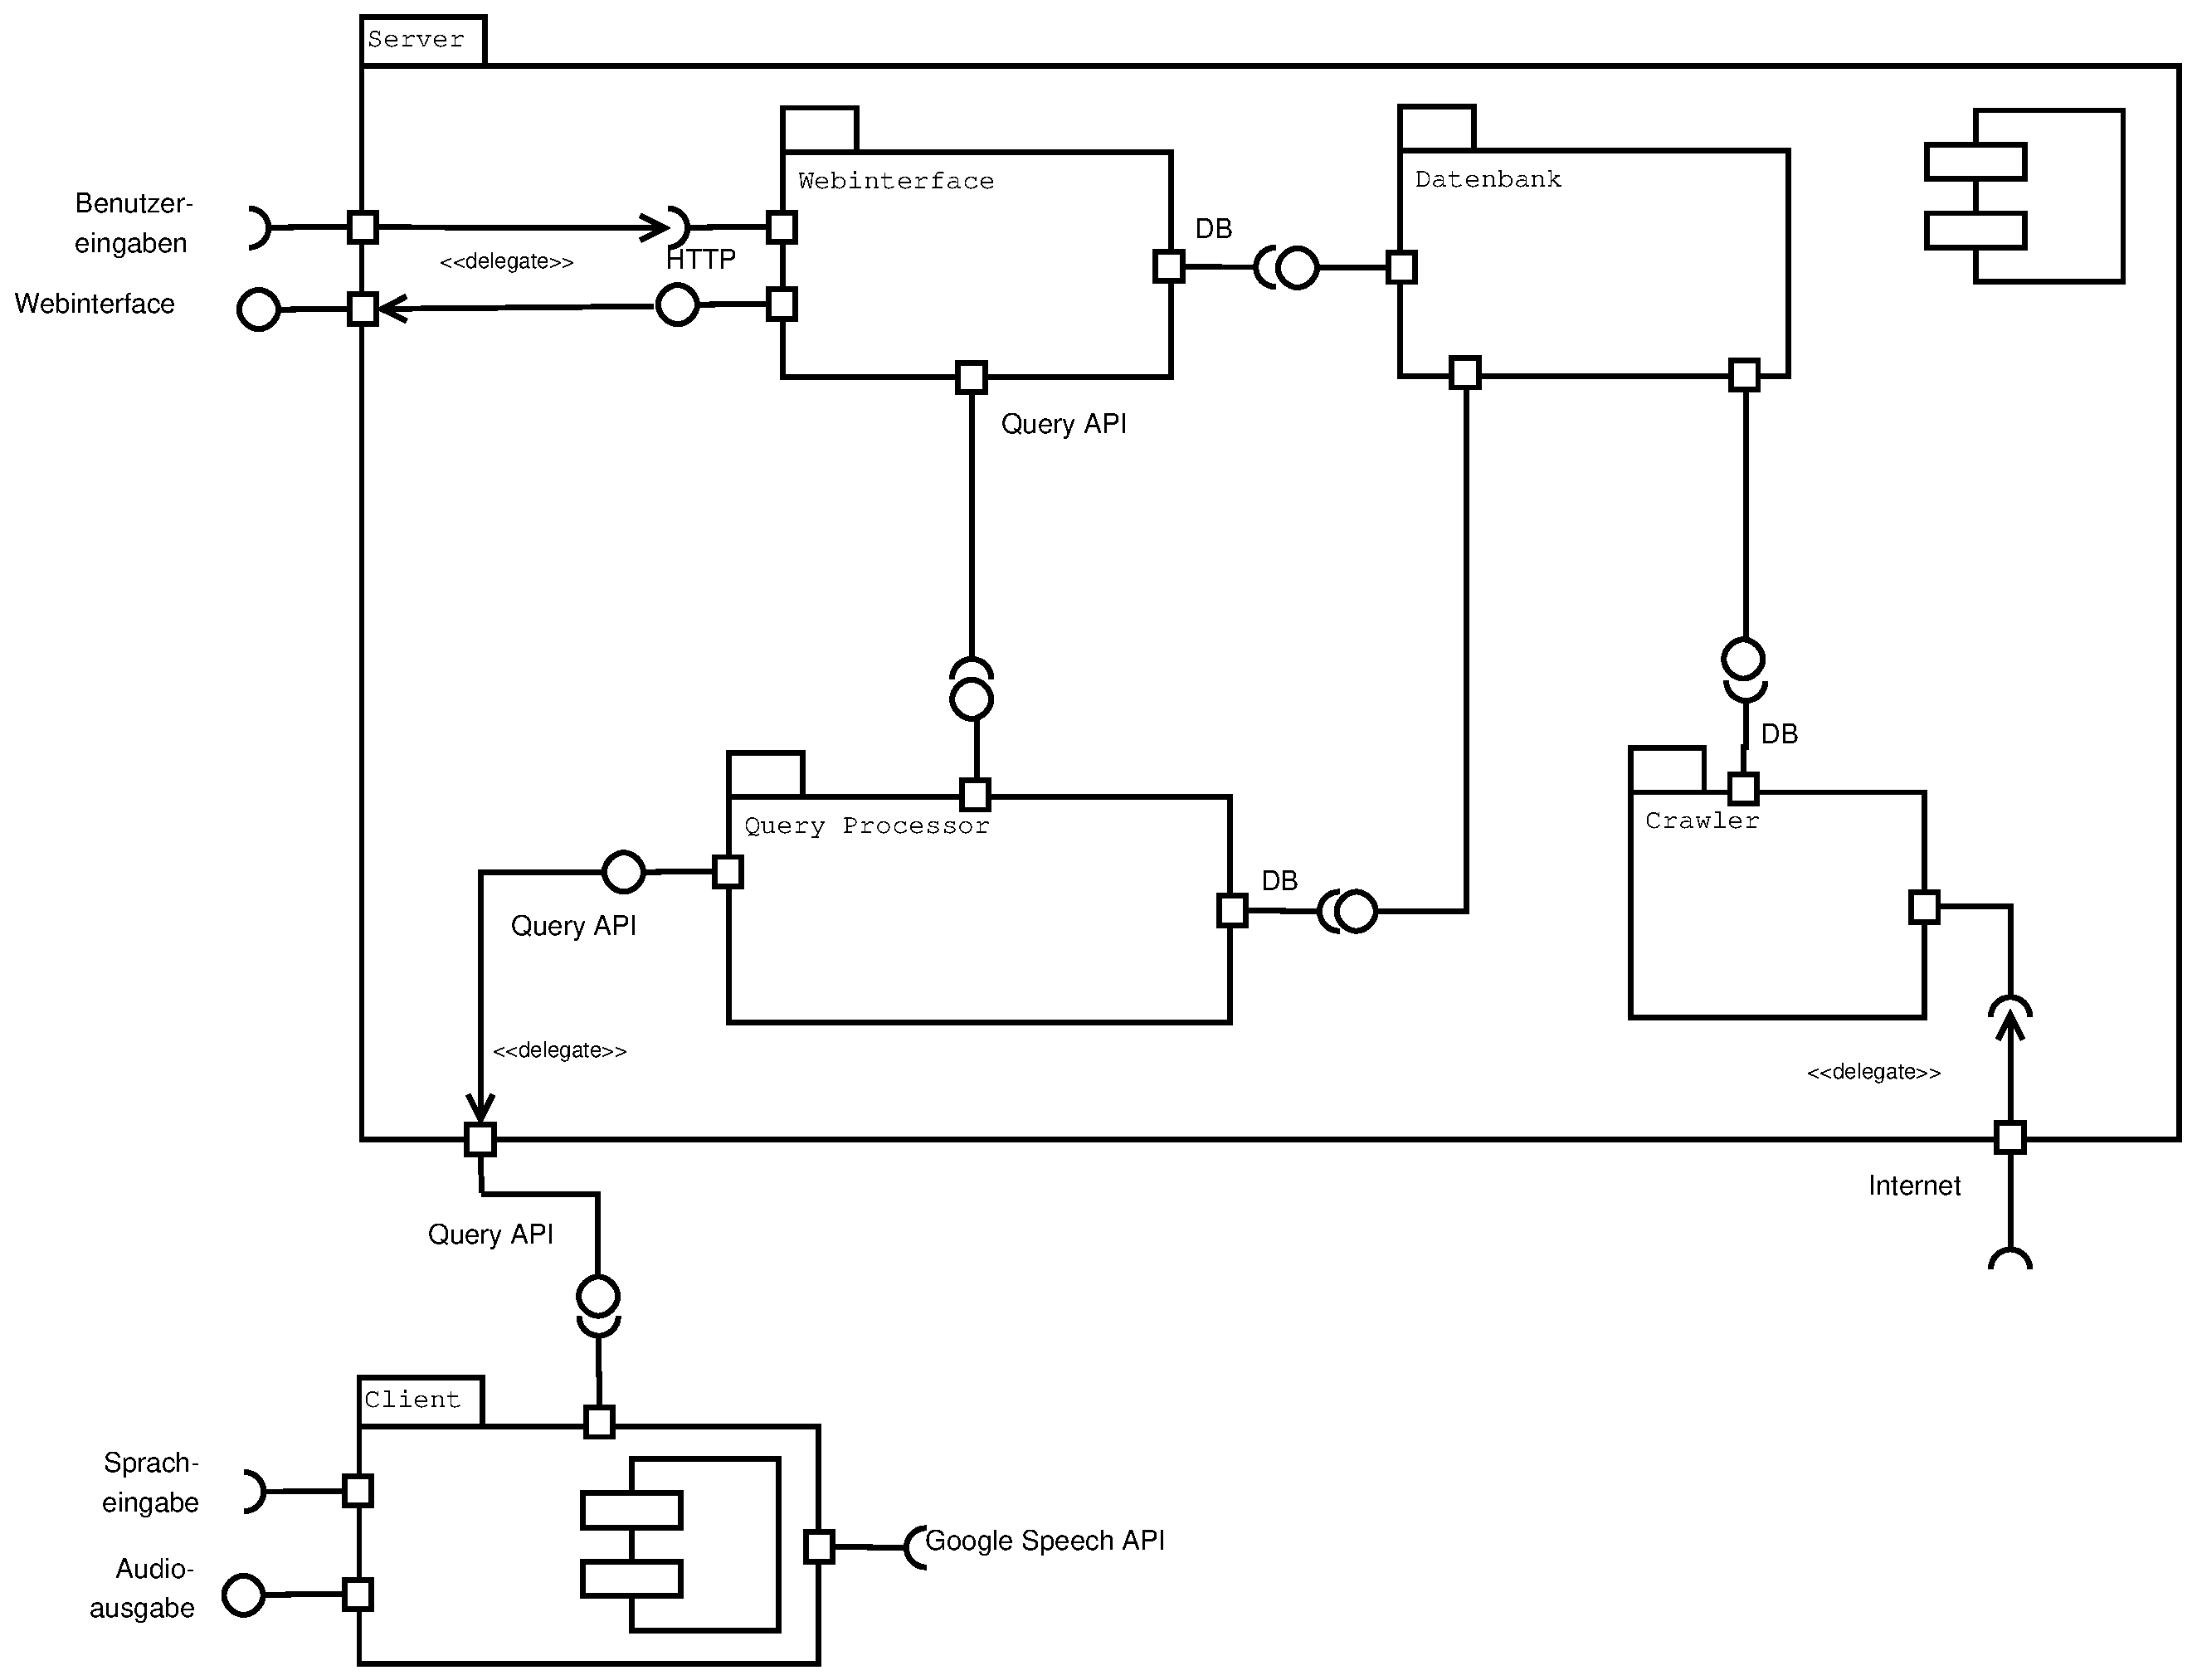
\includegraphics[width=1\textwidth]{Systementwurf/05_implementierungsentwurf/komponenten}
\caption{Komponentendiagramm, \textit{Komponentenaufteilung von \NewsGenie}}
\end{figure}

\begin{figure}[ht]
\centering
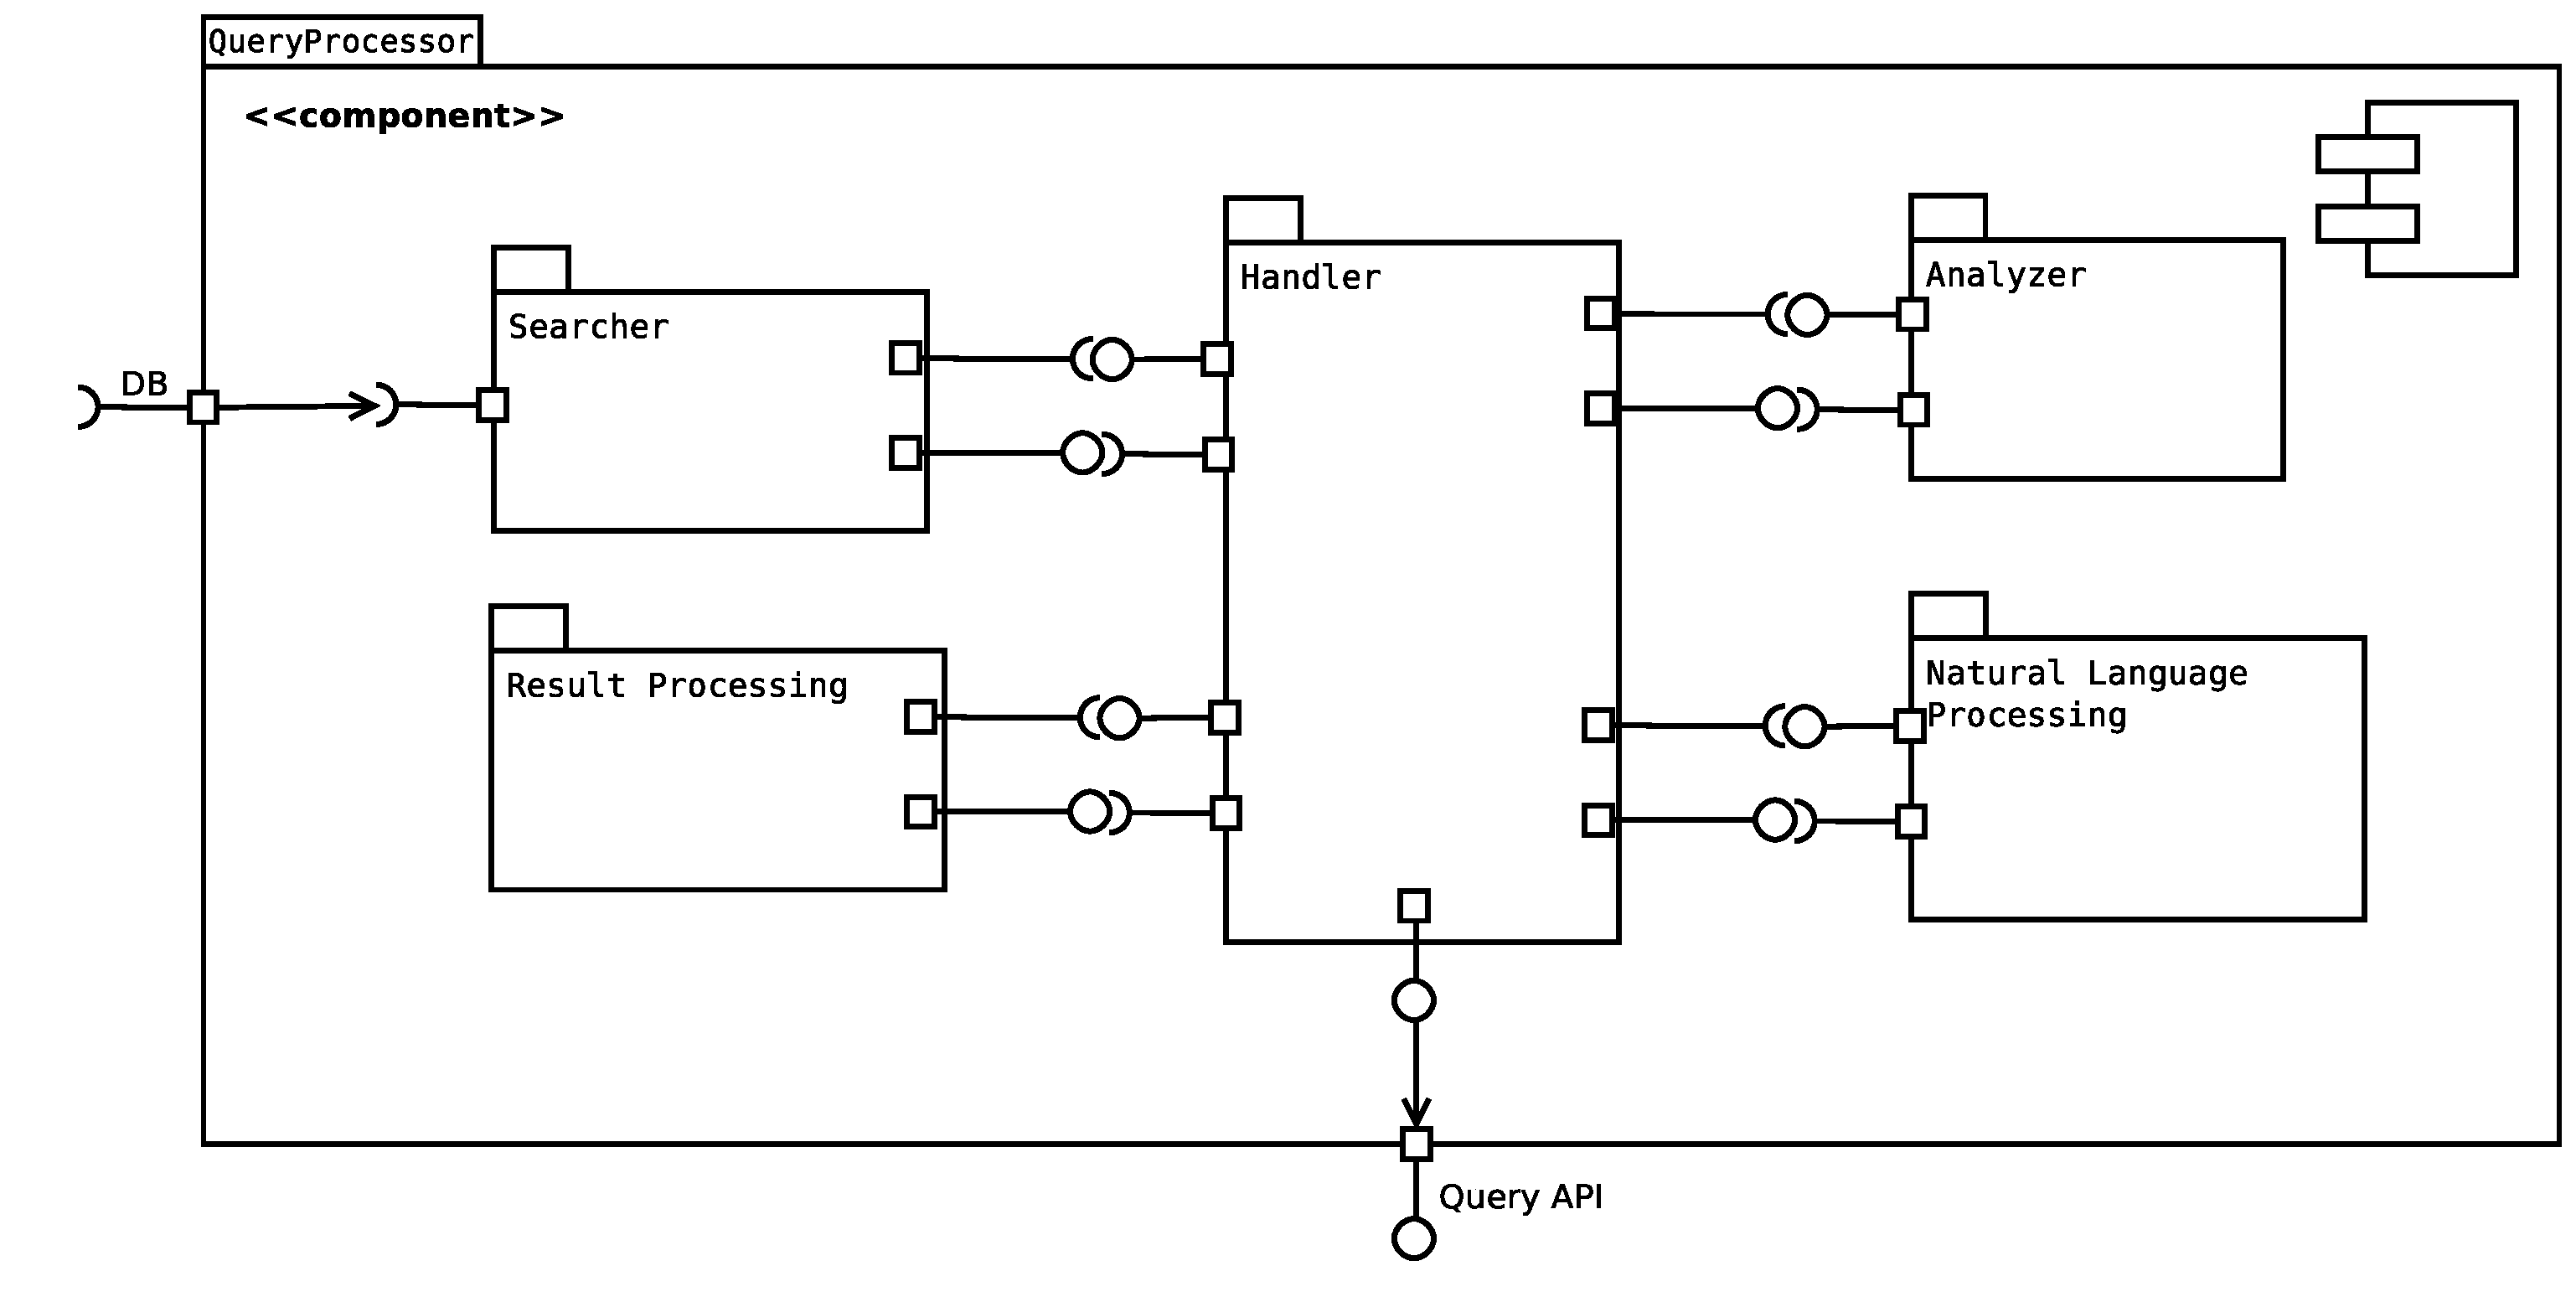
\includegraphics[width=1\textwidth]{Systementwurf/05_implementierungsentwurf/paket-queryprocessor}
\caption{Komponentendiagramm, \textit{Komponenten des Queryprocessors}}
\end{figure}

\FloatBarrier

% C10 Client

\section{Implementierung von Komponente $\langle$C10$\rangle$: Client}

Der Client dient als Frontend des \NewsGenie. Für die Kommunikation mit dem
Server wird das Akka-Framework genutzt. Der Client wird eventbasiert realisiert
und nach dem Start durch den \textit{ServerHandler} gesteuert.

\subsection{Paket-/Klassendiagramm}

\begin{figure}[ht]
\centering
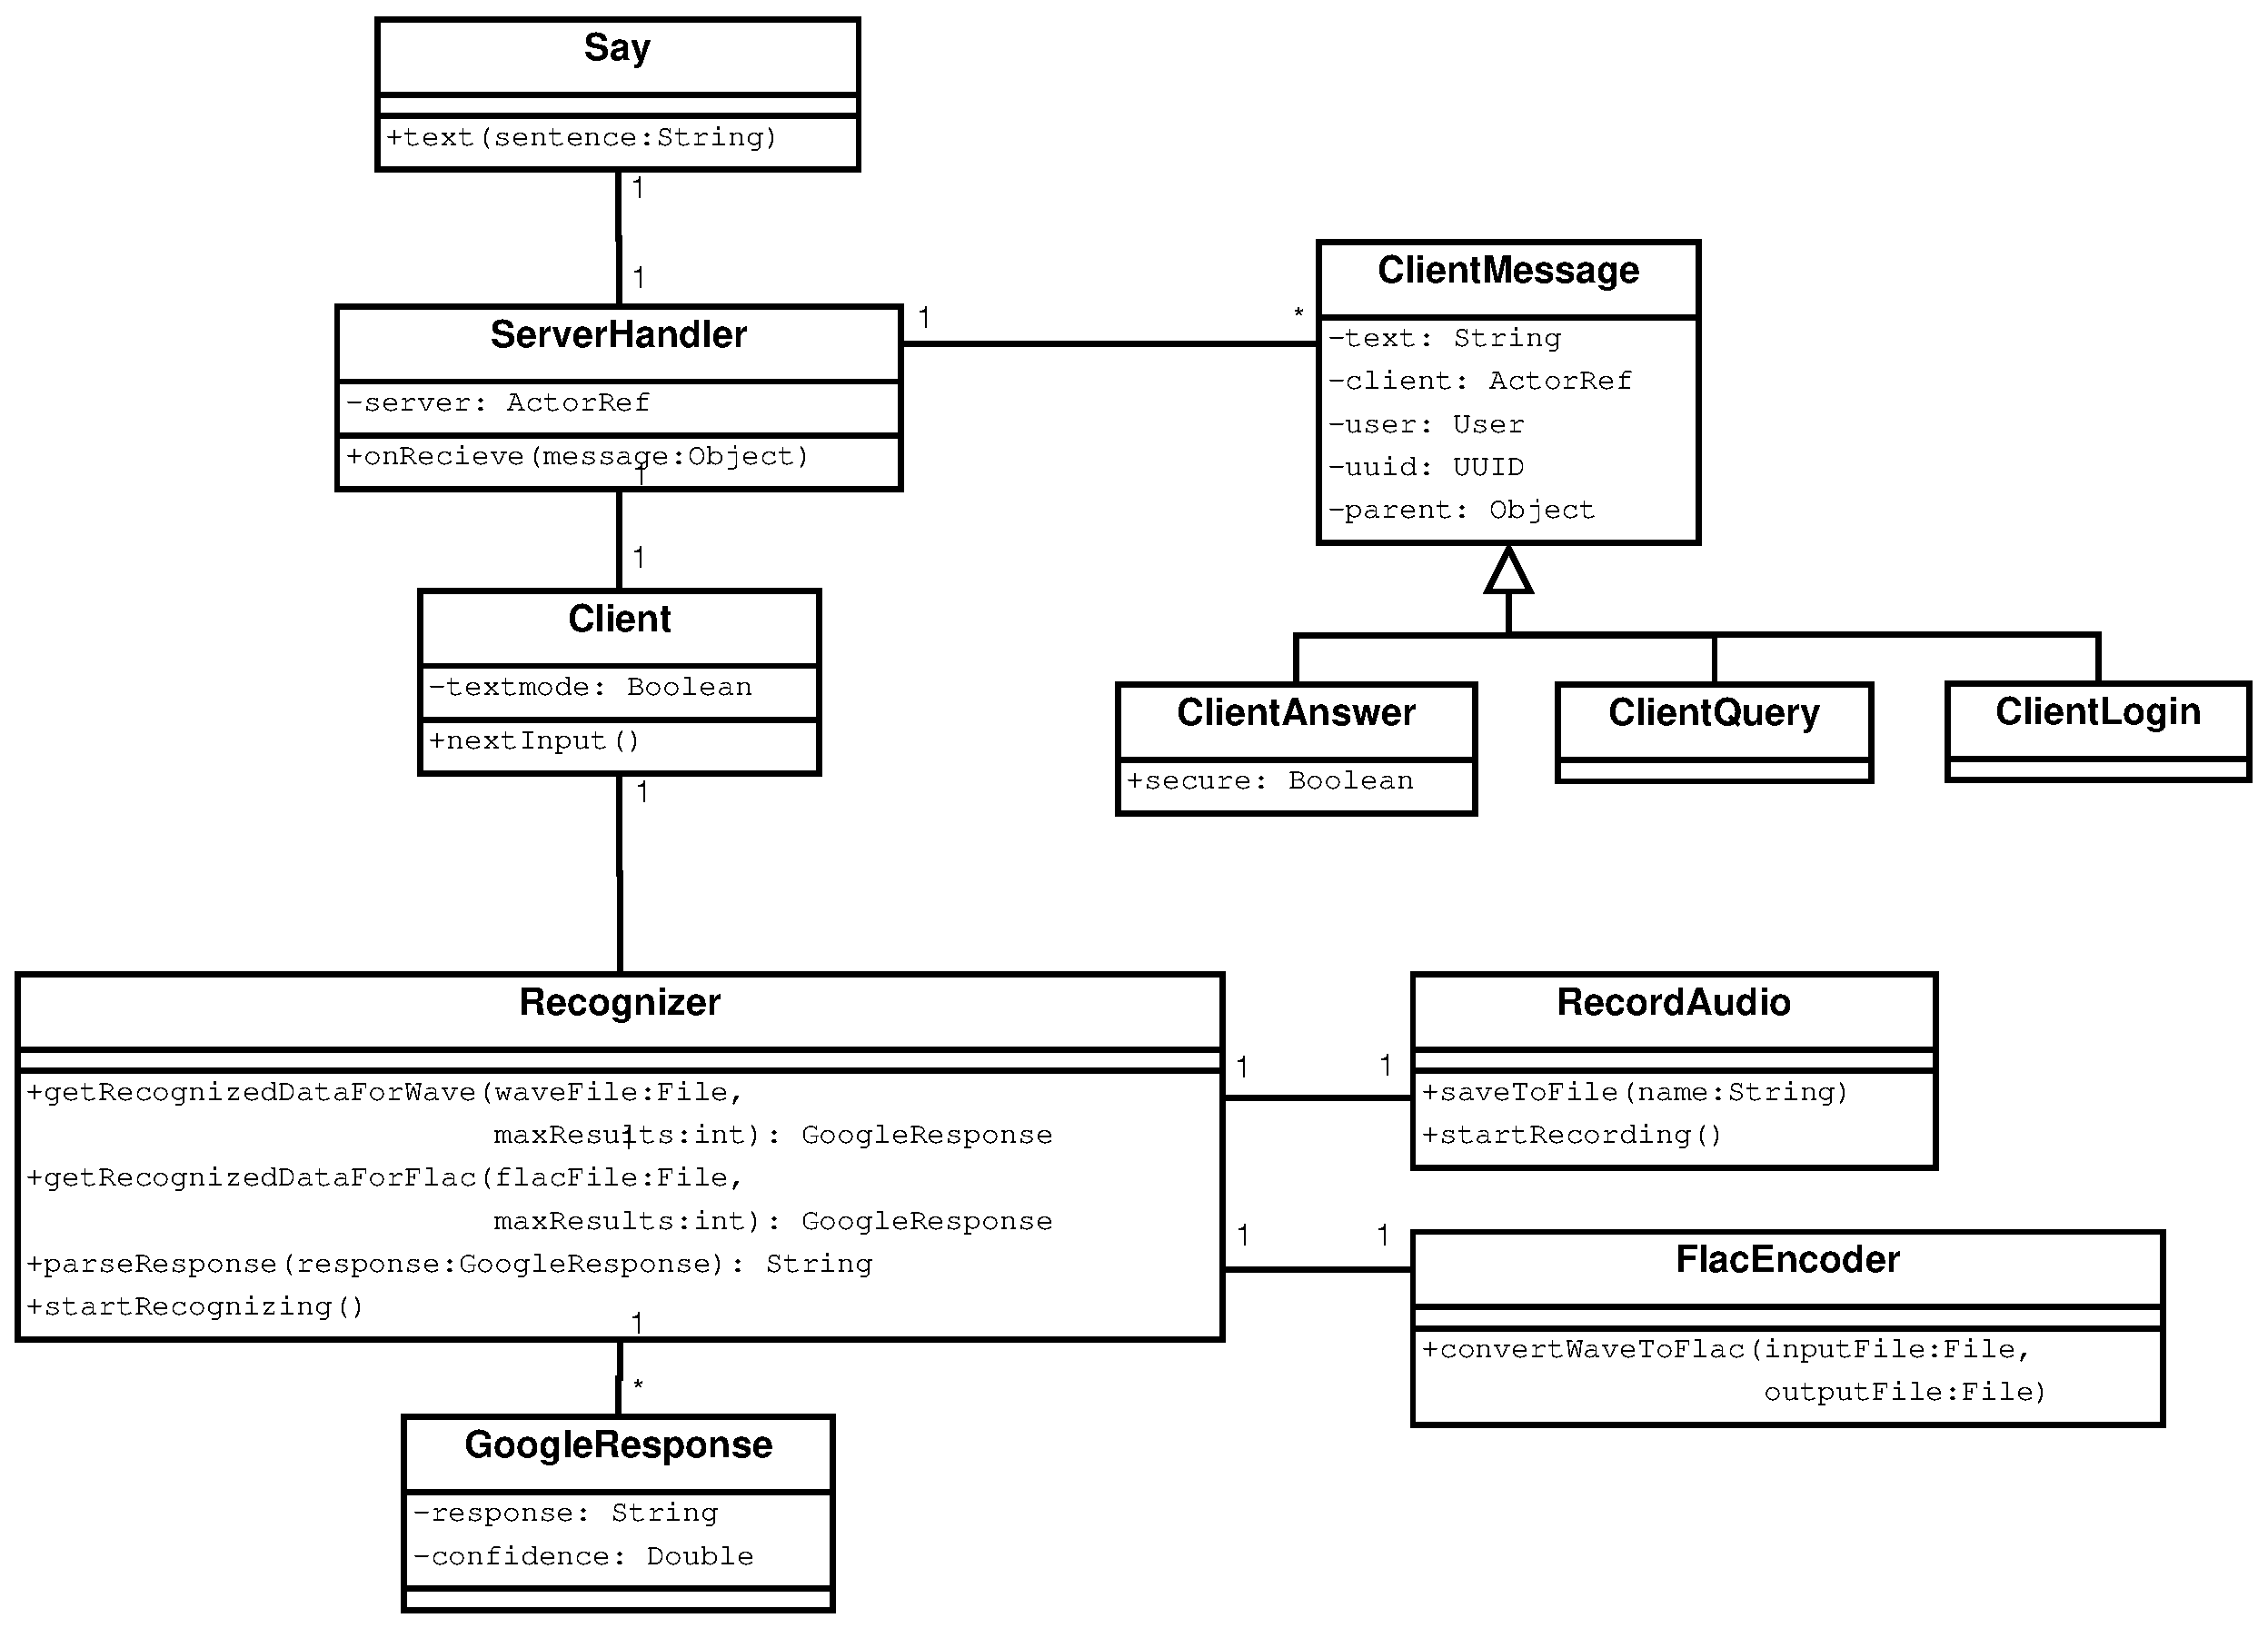
\includegraphics[width=1.03\textwidth]{Systementwurf/05_implementierungsentwurf/client-objekte}
\caption{Klassendiagramm für Komponente \ref{C10}}
\end{figure}

\subsection{Erläuterung}

Im Folgenden werden Attribute, Aufgaben und Kommunikationspartner für jede
Klasse des Clients kurz zu erläutern. Get-/Set-Methoden werden dabei nicht
berücksichtigt, sondern nur deren Attribute als \texttt{private} mit einem
Minuszeichen gekennzeichnet.

\pagebreak[4]
\begin{class}{10}{Client}
\item[Aufgabe]~\
Hauptklasse des Clients. Initialisierung der einzelnen Singleton-Objekte die zum
Bearbeiten einer Anfrage notwendig sind.
\item[Attribute]~\
\begin{itemize}
  \item \texttt{textmode}: falls \texttt{true} akzeptiert der Client
  Tastatureingaben statt Spracheingaben
\end{itemize}
\item[Operationen]~\
\begin{itemize}
  \item \texttt{nextInput()}: startet die nächste Eingabe durch Aufruf des
  \textit{Recognizers}. Der Aufruf erfolgt entweder per Tastendruck oder durch
  den \textit{ServerHandler}.
\end{itemize}
\item[Kommunikationspartner]~\
  \textit{Recognizer}, \textit{ServerHandler}
\end{class}

\begin{class}{10}{Recognizer}
\item[Aufgabe]~\
Realisiert die Umwandlung der Sprachbefehle in Text.
\item[Attribute]~\
keine
\item[Operationen]~\
\begin{itemize}
    \item \texttt{getRecognizedDataForWave(File waveFile, int maxResults)}
    schickt eine Wave-Datei an die Speech-API und erhält ein
    \texttt{GoogleResponse}-Objekt zurück.
    \item \texttt{getRecognizedDataForFlac(File flacFile, int maxResults)}
    schickt eine Flac-Datei an die Speech-API und erhält ein 
    \texttt{GoogleResponse}-Objekt zurück.
    \item \texttt{parseResponse(GoogleResponse response)} wertet ein
    \texttt{GoogleResponse}-Objekt aus und gibt die erkannte Anfrage als String
    zurück.
    \item \texttt{startRecognizing()} steuert den Ablauf einer Anfrage über
    Aufzeichnung und Erkennung und gibt einen String zurück.
\end{itemize}
\item[Kommunikationspartner]~\
\textit{RecordAudio}, \textit{FlacEncoder}, \textit{GoogleResponse}
\end{class}

\begin{class}{10}{RecordAudio}
\item[Aufgabe]~\
Steuert die Audioaufnahme und Speicherung. Diese Klasse ist als Singleton
ausgelegt.
\item[Attribute]~\
keine
\item[Operationen]~\
\begin{itemize}
    \item \texttt{saveToFile(String name)} speichert eine erfolgte Audioaufnahme
    als Wave-Datei.
    \item \texttt{startRecording()} startet die Aufnahme über das Mikrofon,
    bricht ab, wenn der Pegel unter ein Limit fällt.
\end{itemize}
\item[Kommunikationspartner]~\
\textit{Recognizer}
\end{class}

\begin{class}{10}{FlacEncoder}
\item[Aufgabe]~\
Singleton-Klasse zur Umwandlung von Wave in Flac-Dateien.
\item[Attribute]~\
keine
\item[Operationen]~\
\begin{itemize}
    \item \texttt{convertWaveToFlac(File inputFile, File outputFile)} wandelt
    eine Wave-Datei in eine Flac-Datei um.
\end{itemize}
\item[Kommunikationspartner]~\
\textit{Recognizer}
\end{class}

\begin{class}{10}{GoogleResponse}
\item[Aufgabe]~\
Speicherung der Google Speech-API Antwortdaten
\item[Attribute]~\
\begin{itemize}
    \item \texttt{response} Antwort der Speech-API als String
    \item \texttt{confidence} prozentuale Sicherheit der erfolgten Erkennung als
    Double-Wert
\end{itemize}
\item[Operationen]~\
keine
\item[Kommunikationspartner]~\
\textit{Recognizer}
\end{class}

\begin{class}{10}{ServerHandler}
\item[Aufgabe]~\
Singleton-Klasse für die Serverkommunikation. Der Nachrichtenaustausch erfolgt
durch das Senden von Objekten zwischen Server und Client.
\item[Attribute]~\
\begin{itemize}
    \item \texttt{server} Akka-ActorRef-Object, dass auf den Server verweist.
\end{itemize}
\item[Operationen]~\
\begin{itemize}
    \item \texttt{onRecieve(Object message)}
\end{itemize}
\item[Kommunikationspartner]~\
\textit{Client}, \textit{Say}, \textit{ClientMessage}
\end{class}

\begin{class}{10}{Say}
\item[Aufgabe]~\
Singleton-Klasse zur Ausgabe von Text als Sprache.
\item[Attribute]~\
keine
\item[Operationen]~\
\begin{itemize}
    \item \texttt{text(String sentence)} wandelt einen String in eine Wave-Datei
    um und spielt diese ab.
\end{itemize}
\item[Kommunikationspartner]~\

\end{class}

\begin{class}{10}{ClientMessage}
\item[Aufgabe]~\
Superklasse der Nachrichten, die zwischen Server und Client ausgetauscht werden.
\item[Attribute]~\
\begin{itemize}
    \item \texttt{text} Text der Nachricht als String.
    \item \texttt{client} Akka-ActorRef-Objekt mit Verweis auf den absendenden
    Client.
    \item \texttt{user} auf dem Client angemeldeter Benutzer als User-Objekt.
    \item \texttt{uuid} einzigartige ID zur Identifikation der Nachricht.
    \item \texttt{parent} enthält evtl. ein Objekt, dass der Server zur weiteren
    Auswertung mit an den Client übergeben möchte, z.B. eine Liste von Artikeln.
\end{itemize}
\item[Operationen]~\
keine
\item[Kommunikationspartner]~\
\textit{ServerHandler}
\end{class}

\begin{class}{10}{ClientAnswer}
\item[Aufgabe]~\
Objekt zur Übertragung einer Serverantwort an den Client
\item[Attribute]~\
Attribute der Superklasse, sowie
\begin{itemize}
    \item \texttt{secure} Bool'scher Wert, \textit{true} falls die Antwort
    sicher ist und ohne Rückfrage auskommt.
\end{itemize}
\item[Operationen]~\
keine
\item[Kommunikationspartner]~\
\textit{ServerHandler}
\end{class}

\begin{class}{10}{ClientQuery}
\item[Aufgabe]~\
Objekt zur Übertragung einer Clientanfrage an den Server
\item[Attribute]~\
nur Attribute der Superklasse
\item[Operationen]~\
keine
\item[Kommunikationspartner]~\
\textit{ServerHandler}
\end{class}

\begin{class}{10}{ClientLogin}
\item[Aufgabe]~\
Objekt zur Übertragung einer Loginanfrage vom Client zum Server
\item[Attribute]~\
nur Attribute der Superklasse
\item[Operationen]~\
keine
\item[Kommunikationspartner]~\
\textit{ServerHandler}
\end{class}

\FloatBarrier

% C20 Webinterface
%!TEX root = ../../Systementwurf2.tex

\section{Implementierung von Komponente <C20>: Webinterface}

Das Webinterface stellt eine Schnittstelle für Benutzer und Administratoren bereit, in dem sie ihre Einstellungen verwalten können. Es wird mit dem Play-Framework implementiert und kommuniziert mit dem Server eventbasiert mittels Akka.

\subsection{Paket-/Klassendiagramm}

\begin{figure}[ht]
\centering
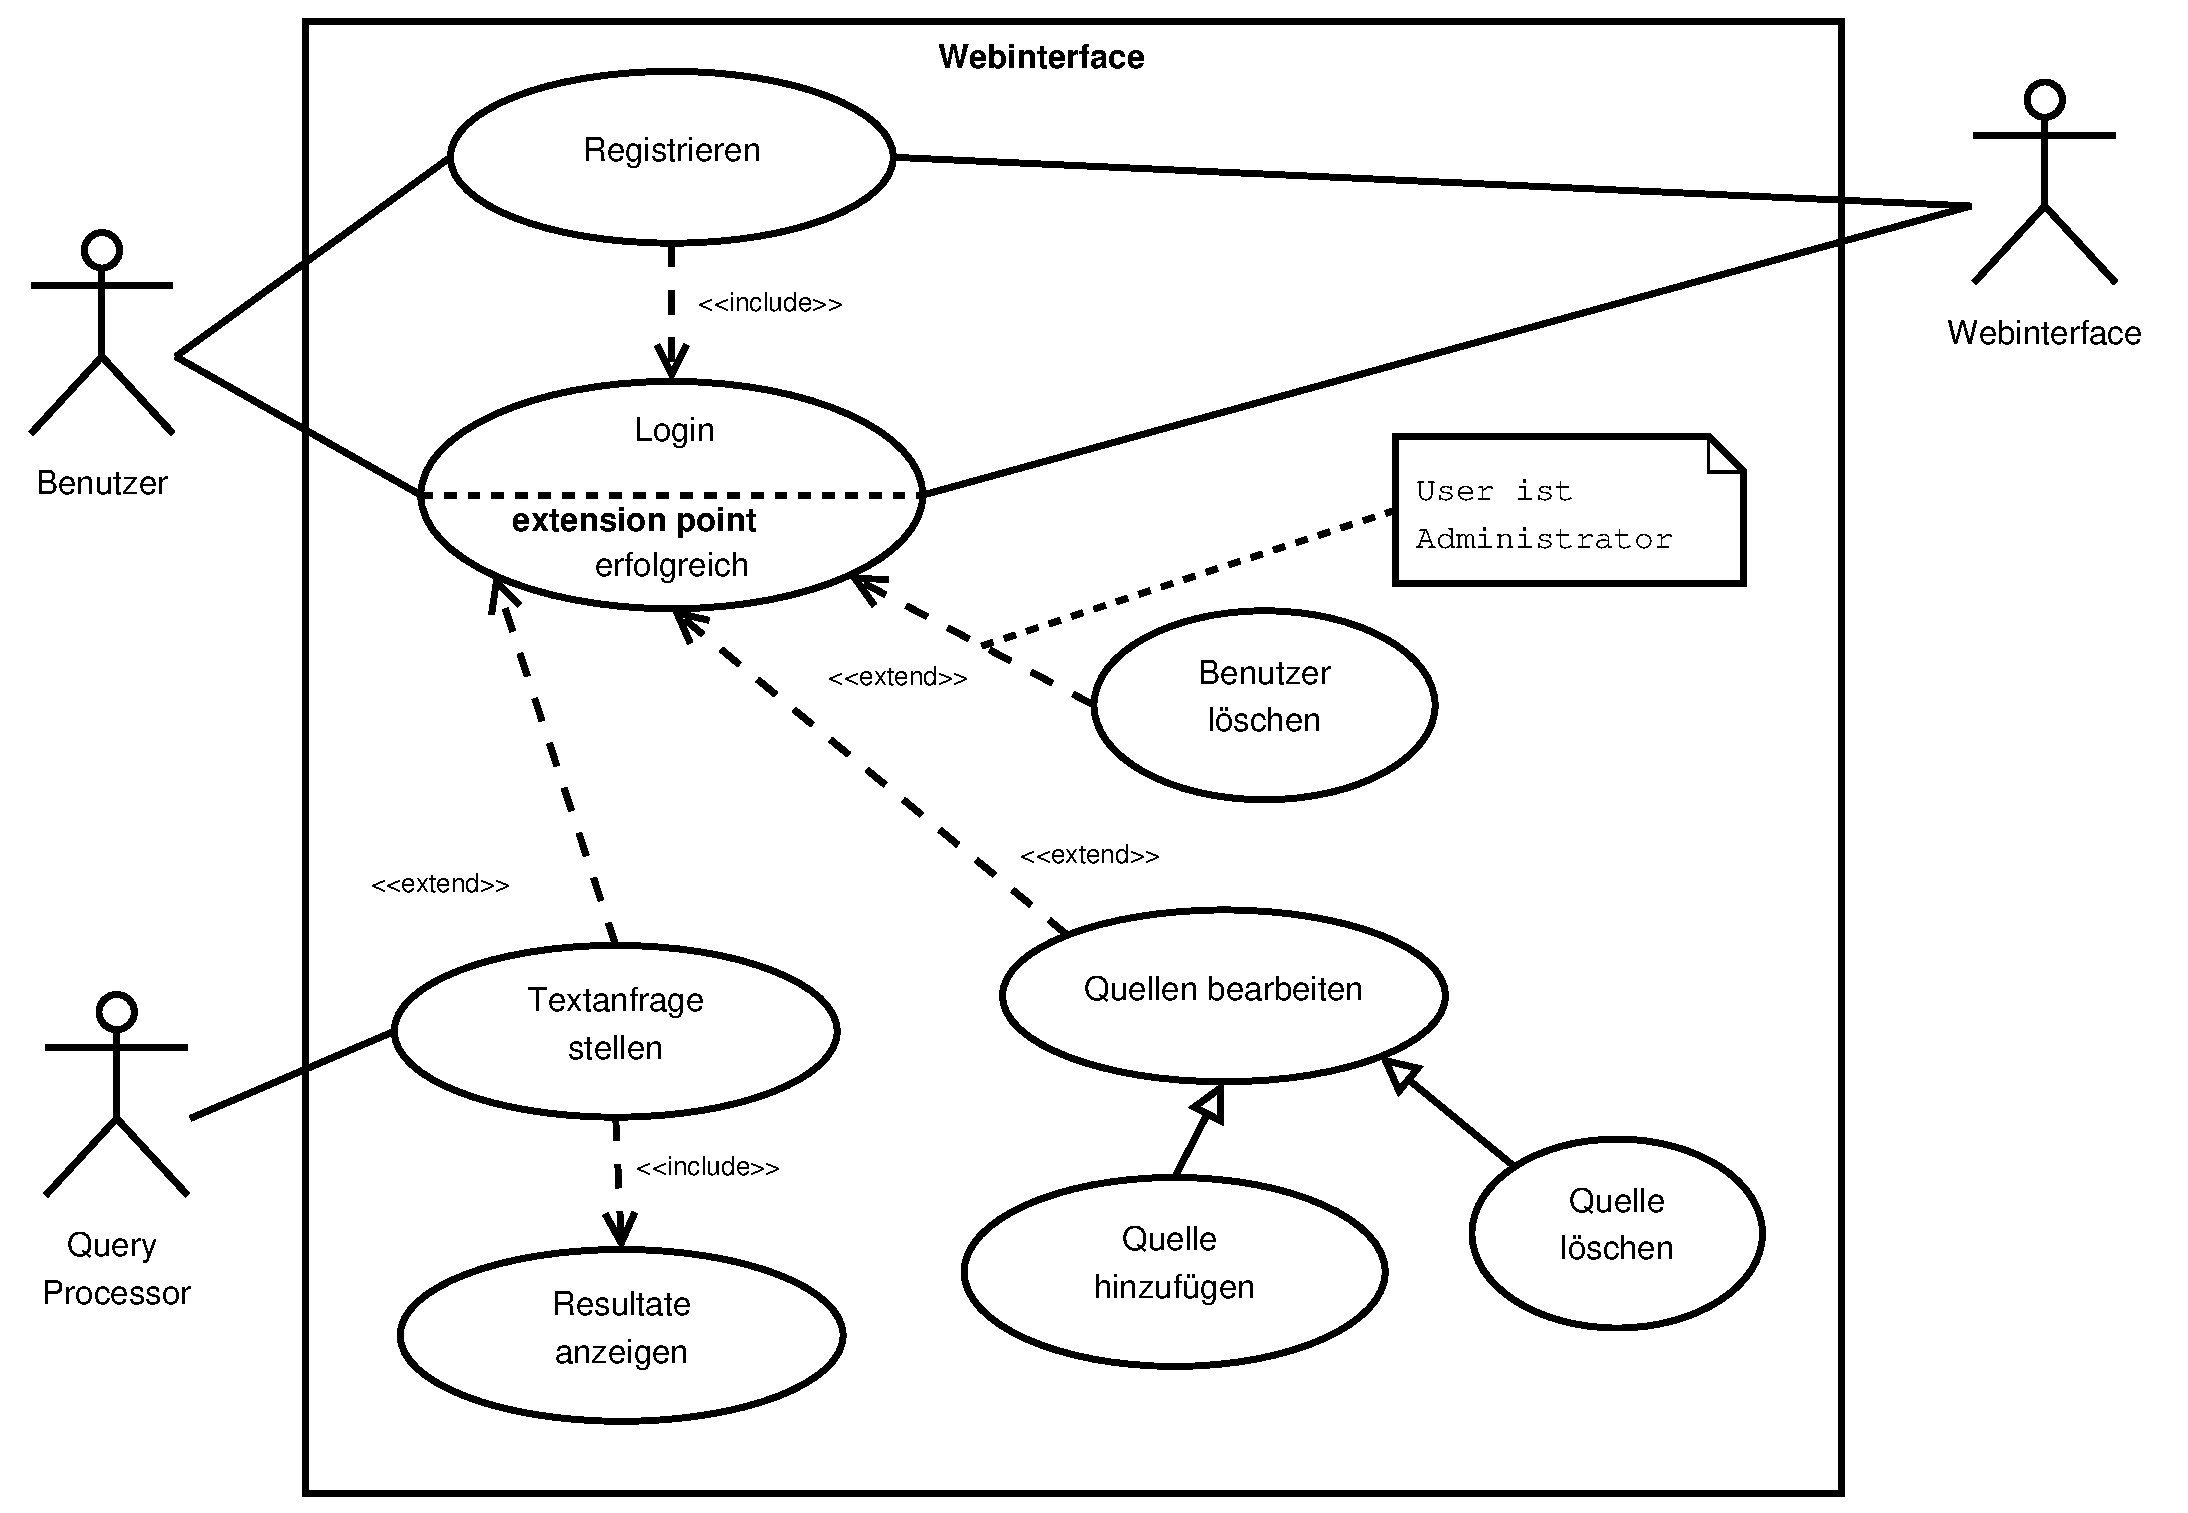
\includegraphics[width=1.03\textwidth]{Systementwurf/05_implementierungsentwurf/webinterface}
\caption{Klassendiagramm für Komponente \ref{C20}}
\end{figure}

\subsection{Erläuterung}

Im Folgenden werden Attribute, Aufgaben und Kommunikationspartner für jede Klasse des Webinterfaces kurz erläutert.\\
Die Funktionen der Klassen (außer Communication) besitzen keine Parameter, da diese per HTTP übertragen werden.

\begin{class}{10}{Communication}
\item[Aufgabe]~\
Die Communication-Klasse ist für die Kommunikation mit dem Server zuständig.
\item[Attribute]~\ keine
\item[Operationen]~\
\begin{itemize}
  \item \texttt{loginRequest(String, String)}: Sendet eine Anfrage, um einen Benutzer einzuloggen.
  \item \texttt{registerRequest(String, String, String)}: Sendet eine Anfrage, um einen neuen Benutzer zu registrieren.
  \item \texttt{userFeedsRequest(User)}: Sendet eine Anfrage, um alle Feeds eines Benutzers zu erhalten.
  \item \texttt{addFeedRequest(User, List<Feed>)}: Sendet eine Anfrage, um einen Benutzer mit Feeds zu verknüpfen.
  \item \texttt{removeFeedRequest(User, List<Feed>)}: Sendet eine Anfrage, um die Verknüpfungen zwischen einem Benutzer und Feeds zu entfernen.
  \item \texttt{userListRequest()}: Sendet eine Anfrage, um eine Liste aller Benutzer zu erhalten.
  \item \texttt{deleteUserRequest(User)}: Sendet eine Anfrage, um einen Benutzer zu löschen.
  \item \texttt{changeAdminRequest(User)}: Sendet eine Anfrage, um einem Benutzer Administratorenrechte zu gewähren oder zu entziehen.
  \item \texttt{createFeedRequest(Feed)}: Sendet eine Anfrage, um einen neuen Feed anzulegen.
  \item \texttt{deleteFeedRequest(Feed)}: Sendet eine Anfrage, um einen Feed zu löschen.
\end{itemize}
\item[Kommunikationspartner]~\
  \textit{ServerHandler}
\end{class}

\begin{class}{20}{AdminFeeds}
\item[Aufgabe]~\
Die AdminFeeds-Klasse stellt die Webseite zum Administrieren von Feeds zur Verfügung.
\item[Attribute]~\ keine
\item[Operationen]~\
\begin{itemize}
    \item \texttt{showFeedsControl()} Zeigt die Webseite an.
    \item \texttt{addFeed()} Sendet eine Anfrage, einen neuen Feed zu erstellen.
    \item \texttt{deleteFeed()} Sendet eine Anfrage, einen Feed zu löschen.
\end{itemize}
\item[Kommunikationspartner]~\ keine
\end{class}

\begin{class}{30}{AdminUser}
\item[Aufgabe]~\
Die AdminUser-Klasse stellt die Webseite zum Administrieren von Benutzern zur Verfügung.
\item[Attribute]~\ keine
\item[Operationen]~\
\begin{itemize}
    \item \texttt{showUserControl()} Zeigt die Webseite an.
    \item \texttt{userAction()} Löscht einen Benutzer oder ändert seinen Admin-Status.
\end{itemize}
\item[Kommunikationspartner]~\ keine
\end{class}

\begin{class}{40}{Settings}
\item[Aufgabe]~\
Die Settings-Klasse stellt die Webseite zum Ändern der Benutzereinstellungen zur Verfügung.
\item[Attribute]~\ keine
\item[Operationen]~\
\begin{itemize}
    \item \texttt{showSettings()} Zeigt die Webseite an.
    \item \texttt{changePassword()} Sendet eine Anfrage, das Passwort zu ändern.
    \item \texttt{changeLanguage()} Sendet eine Anfrage, die Sprache zu ändern.
\end{itemize}
\item[Kommunikationspartner]~\ keine
\end{class}

\begin{class}{50}{Query}
\item[Aufgabe]~\
Die Query-Klasse stellt die Webseite zum Stellen eines Text-Queries zur Verfügung.
\item[Attribute]~\ keine
\item[Operationen]~\
\begin{itemize}
    \item \texttt{showQueryl()} Zeigt die Webseite an.
    \item \texttt{runQuery()} Sendet eine Anfrage mit einem Text-Query.
\end{itemize}
\item[Kommunikationspartner]~\ keine
\end{class}

\begin{class}{60}{Feeds}
\item[Aufgabe]~\
Die Feeds-Klasse stellt die Webseite zum Verwalten der Feedeinstellungen zur Verfügung.
\item[Attribute]~\ keine
\item[Operationen]~\
\begin{itemize}
    \item \texttt{showFeedsl()} Zeigt die Webseite an.
    \item \texttt{subscribe()} Sendet eine Anfrage, Feeds zu abonnieren.
    \item \texttt{dleteFeed()} Sendet eine Anfrage, Feeds zu deabonnieren.
\end{itemize}
\item[Kommunikationspartner]~\ keine
\end{class}

\begin{class}{70}{Application}
\item[Aufgabe]~\
Die Application-Klasse stellt die Startwebseite zur Verfügung.
\item[Attribute]~\ keine
\item[Operationen]~\
\begin{itemize}
    \item \texttt{index()} Zeigt die Startseite an.
\end{itemize}
\item[Kommunikationspartner]~\ keine
\end{class}

\begin{class}{80}{Login}
\item[Aufgabe]~\
Die Login-Klasse stellt die Webseite zum Einloggen zur Verfügung.
\item[Attribute]~\ keine
\item[Operationen]~\
\begin{itemize}
    \item \texttt{showLogin()} Zeigt die Webseite an.
    \item \texttt{login()} Sendet eine Anfrage, einen Benutzer einzuloggen.
    \item \texttt{logout()} Sendet eine Anfrage, einen Benutzer auszuloggen.
\end{itemize}
\item[Kommunikationspartner]~\ keine
\end{class}

\begin{class}{90}{Register}
\item[Aufgabe]~\
Die Register-Klasse stellt die Webseite zum Registrieren zur Verfügung.
\item[Attribute]~\ keine
\item[Operationen]~\
\begin{itemize}
    \item \texttt{showRegister()} Zeigt die Webseite an.
    \item \texttt{register()} Sendet eine Anfrage, einen neuen Benutzer zu registrieren.
\end{itemize}
\item[Kommunikationspartner]~\ keine
\end{class}

\begin{class}{100}{Recovery}
\item[Aufgabe]~\
Die Recovery-Klasse stellt die Webseite zum Wiederherstellen des Passworts zur Verfügung.
\item[Attribute]~\ keine
\item[Operationen]~\
\begin{itemize}
    \item \texttt{showRecovery()} Zeigt die Webseite an.
    \item \texttt{recover()} Sendet eine Anfrage, das Passwort wiederherzustellen.
\end{itemize}
\item[Kommunikationspartner]~\ keine
\end{class}

% C30 Datenbank
%!TEX root = ../../Systementwurf2.tex

\section{Implementierung von Komponente <C30>: Datenbank}

Die Datenbankkomponente dient zur Kommunikation mit dem Virtuoso Triplestore und dem Apache Lucene Index. Die Kommunikation mit den anderen Komponenten erfolgt eventbasiert mit Hilfe des Akka-Frameworks.

\subsection{Paket-/Klassendiagramm}

\begin{figure}[ht]
\centering
\includegraphics[width=1.03\textwidth]{Systementwurf/05_implementierungsentwurf/database}
\caption{Klassendiagramm für Komponente \ref{C30}}
\end{figure}

\subsection{Erläuterung}

Im Folgenden werden Attribute, Aufgaben und Kommunikationspartner für jede
Klasse der Datenbankkomponente kurz erläutert.

\begin{class}{10}{DatabaseHandler}
\item[Aufgabe]~\
Die DatabaseHandler-Klasse ist die Hauptklasse der Datenbankkomponente. Sie nimmt Anfragen der anderen Komponenten mittels der onReceive() Methode entgegen und sendet Antworten auf diese Anfragen.
\item[Attribute]~\
\begin{itemize}
  \item \texttt{connection}: Referenz auf den \textit{DatabaseConnection}-Singleton.
  \item \texttt{index}: Referenz auf ein \textit{Index}-Objekt.
  \item \texttt{lod}: Referenz auf den \textit{LinkedOpenData}-Singleton.
\end{itemize}
\item[Operationen]~\
\begin{itemize}
  \item \texttt{onReceive()}: nimmt Anfragen anderer Komponenten entgegen und beantwortet sie.
\end{itemize}
\item[Kommunikationspartner]~\
  \textit{DatabaseConnection}, \textit{Index}, \textit{LinkedOpenData}, \textit{Searcher}, \textit{CrawlerHandler}, \textit{ManagementHandler}
\end{class}

\begin{class}{20}{DatabaseConnection}
\item[Aufgabe]~\
Die DatabaseConnection-Klasse enthält die verschiedenen SPARQL-Queries an den Virtuoso-Triplestore.
\item[Attribute]~\
\begin{itemize}
  \item \texttt{instance}: Referenz auf den \textit{DatabaseConnection}-Singleton.
  \item \texttt{url}: URL unter der die Virtuoso-Datenbank erreicht werden kann.
  \item \texttt{graphName}: Name des RDF-Graphen auf dem gearbeitet wird.
  \item \texttt{user}: Virtuoso-Benutzername.
  \item \texttt{pw}: Virtuoso-Benutzerpasswort.
  \item \texttt{prefix}: Prefix für URI Graphenknoten.
  \item \texttt{queryPrefix}: Prefix für URI Graphenknoten in Queries.
  \item \texttt{graph}: Referenz auf den RDF-Graphen auf dem gearbeitet wird.
\end{itemize}
\item[Operationen]~\
\begin{itemize}
    \item \texttt{getInstance()}  Liefert die Singleton-Instanz.
    \item \texttt{addUser(String, String, String)} Legt einen neuen Benutzer in der Datenbank an.
    \item \texttt{getUserByName(String)} Liefert den Benutzer mit dem angegebenen Namen.
    \item \texttt{getAllUsers()} Liefert alle exisistierenden Benutzer.
    \item \texttt{deleteUser(User)} Löscht den angegebenen Benutzer.
    \item \texttt{addFeed(String, String, String)} Legt einen neuen Feed in der Datenbank an.
    \item \texttt{addFeed(Feed)} Legt einen neuen Feed in der Datenbank an.
    \item \texttt{getFeedsOfUser(User)} Liefert die Feeds, die der angegebene Benutzer abonniert hat.
    \item \texttt{getAllFeeds()} Liefert alle existierenden Feeds.
    \item \texttt{deleteFeed(Feed)} Löscht den angegebenen Feed.
    \item \texttt{addArticle(String, String, String, Feed)} Legt einen neuen Artikel in der Datenbank an.
    \item \texttt{addArticle(Article)} Legt einen neuen Artikel in der Datenbank an.
    \item \texttt{getallArticles()} Liefert alle existierenden Artikel.
    \item \texttt{linkUserToFeed(User, List<Feed>)} Verknüpft den angegebenen Benutzer mit den Feeds aus der Liste.
    \item \texttt{unlinkUserFromFeed(User, List<Feed>)} Löscht die Verknüpfungen zwischen dem angegebenen Benutzer und den Feeds aus der Liste.
    \item \texttt{updateLoginDate(User)} Ändert das Datum des letzten Logins des angegebenen Benutzers auf die momentane Zeit.
    \item \texttt{checkPassword(User, String)} Prüft, ob der angegebene Benutzer das angegebene Passwort verwendet.
    \item \texttt{changeAdmin(User)} Ändert den Admin-Status des angegebenen Benutzers.
    \item Hilfsfunktionen: Die Klasse enthält einige private Hilfsfunktionen, die hier nicht näher erläutert werden.
\end{itemize}
\item[Kommunikationspartner]~\
\textit{DatabaseHandler}, \textit{Index}
\end{class}

\begin{class}{30}{Index}
\item[Aufgabe]~\
Die Index-Klasse verwaltet den Apache Lucene Volltextindex.
\item[Attribute]~\
\begin{itemize}
  \item \texttt{analyzer}: Legt fest, welcher Lucene-Analyzer verwendet wird.
  \item \texttt{index}: Ordner, in dem sich der Index im Dateisystem befindet.
  \item \texttt{luceneVersion}: Legt fest, welche Lucene Version verwendet wird.
  \item \texttt{connection}: Referenz auf den \textit{DatabaseConnection}-Singleton.
\end{itemize}
\item[Operationen]~\
\begin{itemize}
    \item \texttt{createIndex()}  Schreibt den Index neu. Dies ist nach jedem Durchlauf des Crawlers notwendig.
    \item \texttt{addDocument(IndexWriter, Article)} Hilfsfunktion von \texttt{createIndex()}.
    \item \texttt{query(Map<String, Float>, List<String>, User)} Stellt einen Query an den Index.
    \item \texttt{generateQuery(Map<String, Float>, List<String>, User)} Hilfsfunktion von\\ \texttt{query(Map<String, Float>, List<String>, User)}.
\end{itemize}
\item[Kommunikationspartner]~\
\textit{DatabaseHandler}, \textit{DataBaseConnection}
\end{class}

\begin{class}{30}{NoFeedsException}
\item[Aufgabe]~\
Intern verwendete Exception, die auftritt, wenn ein Benutzer keine Feeds aboniert hat.
\item[Attribute]~\ keine
\item[Operationen]~\ keine
\item[Kommunikationspartner]~\ keine
\end{class}


% C40 Crawler
\section{Implementierung von Komponente <C40>: Crawler}

Der Crawler dient als Informationslieferant des \NewsGenies. Für die
Kommunikation mit der Datenbank wird das Akka-Framework genutzt. Der Crawler
ruft bei Start eines Crawl-Durchlaufs die Liste der Feeds von der Datenbank
ab und wiederholt diese Operation solange der Server läuft.

\subsection{Paket-/Klassendiagramm}

\begin{figure}[ht]
\centering
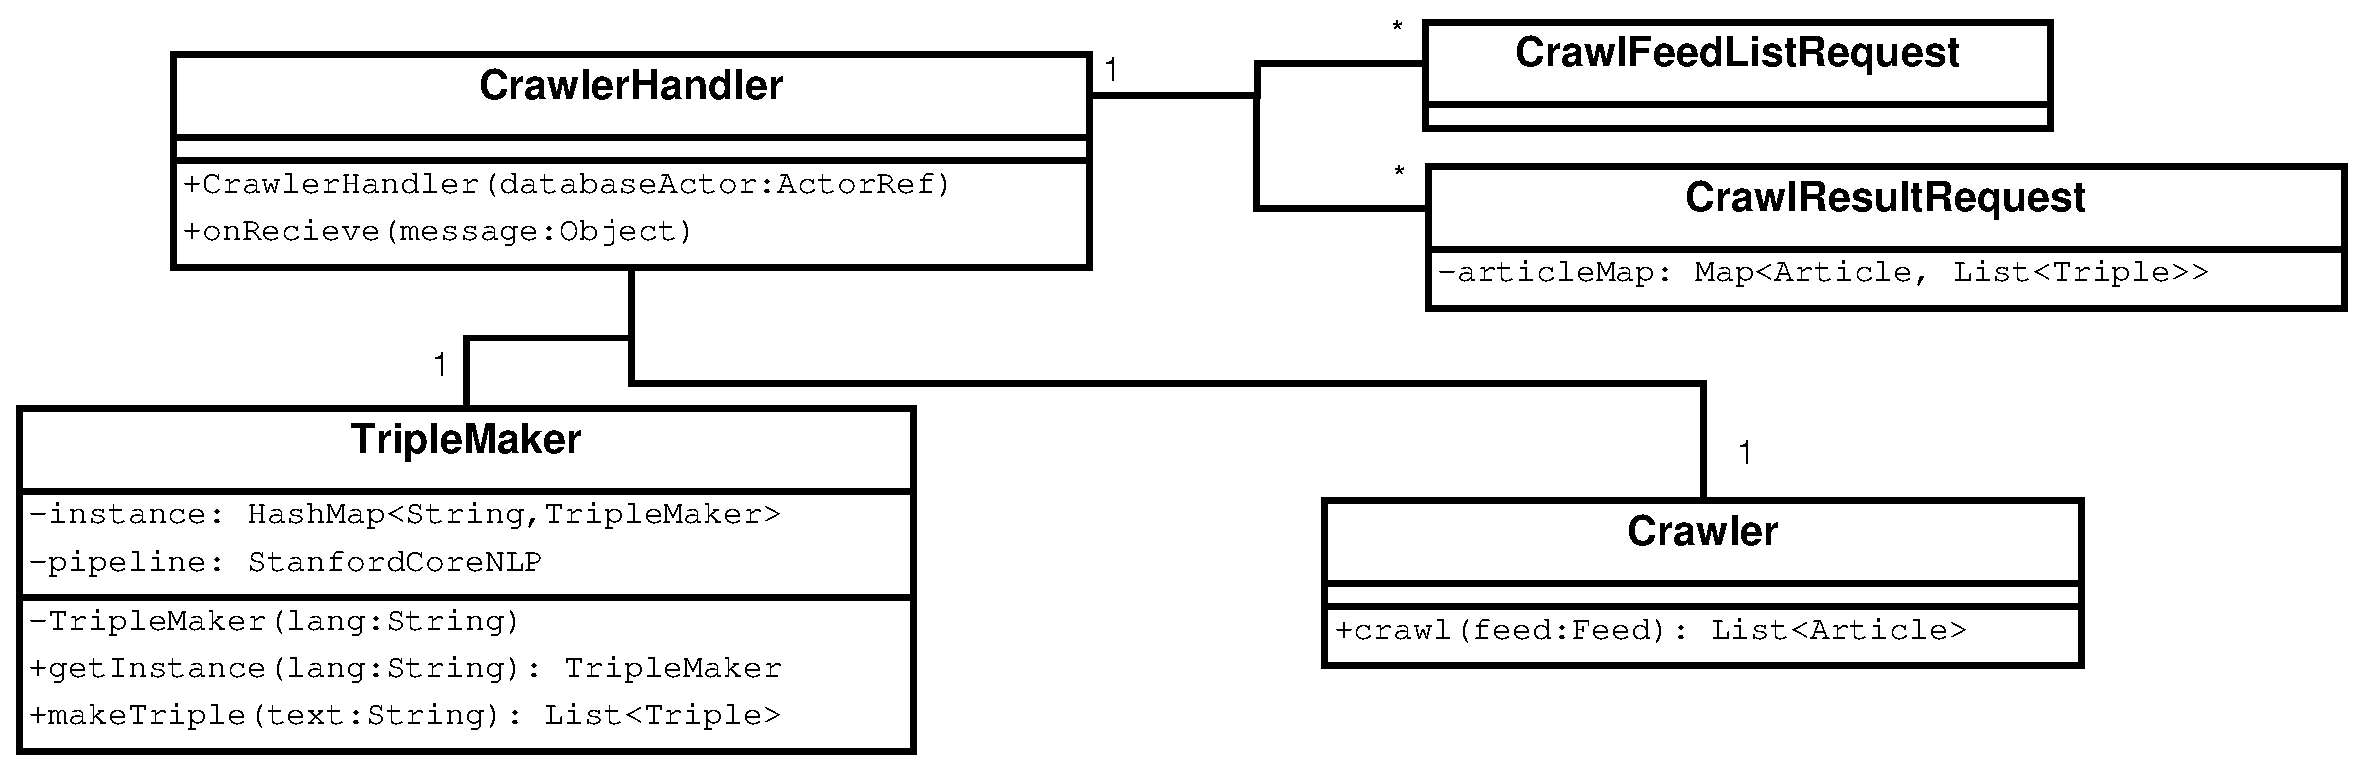
\includegraphics[width=1.03\textwidth]{Systementwurf/05_implementierungsentwurf/crawler-objekte}
\caption{Klassendiagramm für Komponente \ref{C10}}
\end{figure}
 
\subsection{Erläuterung}

Im Folgenden werden Attribute, Aufgaben und Kommunikationspartner für jede
Klasse der Serverkomponenten kurz erläutert. Triviale Methoden werden dabei
nicht berücksichtigt, sondern nur deren Attribute als \texttt{private} mit einem
Minuszeichen gekennzeichnet.

\begin{class}{40}{CrawlerHandler}
\item[Aufgabe]~\
Hauptklasse des Crawlers. Initialisierung der einzelnen Singleton-Objekte die
zum Bearbeiten eines Crawlvorgangs notwendig sind.
\item[Attribute]~\
\begin{itemize}
  \item \texttt{tripleMaker}: TripleMaker-Instanz
  \item \texttt{crawler}: Crawler-Instanz
  \item \texttt{databaseActor}: Akka-ActorRef-Objekt mit Verweis auf den
  DatabaseHandler
\end{itemize}
\item[Operationen]~\
\begin{itemize}
  \item \texttt{CrawlerHandler(ActorRef databaseActor)}:
  Instanziert die unter Attribute genannten Werte und sendet der
  Datenbank ein CrawlFeedListRequest. 
  \item \texttt{onRecive(Object message)}: Behandlet die eingehenden Messages:
\end{itemize}
\item[Kommunikationspartner]~\
  \textit{DatabaseHandler}
\end{class}

\begin{class}{40}{Crawler}
\item[Aufgabe]~\
Singleton-Klasse für das Crawlen der FeedList.
\item[Attribute]~\
keine
\item[Operationen]~\
\begin{itemize}
    \item \texttt{crawl(Feed feed)}: Crawlt von dem übergebenen Feed den Inhalt
    und lädt den Artikeltext.
\end{itemize}
\item[Kommunikationspartner]~\
\textit{CrawlerHandler}
\end{class}

\begin{class}{40}{TripleMaker}
\item[Aufgabe]~\
Singleton-Klasse für das Zerteilen der Artikeltexte in Triple für die Datenbank.
\item[Attribute]~\
\begin{itemize}
  \item \texttt{instance}: \texttt{TripleMaker}-Instanz für die verschiedenen 
  \item \texttt{pipeline}: \texttt{StandfortCoreNLP}-Instanz
  \item \texttt{lang}: Speichert die Sprache für die Triplezerlegung
\end{itemize}
\item[Operationen]~\
\begin{itemize}
    \item \texttt{TripleMaker(String lang)}: Instanziert die texttt{pipeline}
    mit den passenden Spracheinstellungen.
    \item \texttt{getInstance(String lang)}: Instanziert den texttt{TripleMaker}
    oder gibt eine schon bestehende Instanz zurück.
    \item \texttt{makeTriple(String text)}: Zerlegt den übergebenen Text in
    Triple.
\end{itemize}
\item[Kommunikationspartner]~\
\textit{CrawlerHandler}
\end{class}

\begin{class}{40}{CrawlFeedListRequest}
\item[Aufgabe]~\
Objekt zur Anfrage auf Erhalt der Feedliste.
\item[Attribute]~\
keine
\item[Operationen]~\
keine
\item[Kommunikationspartner]~\
\textit{DatabaseHandler}
\end{class}

\begin{class}{40}{CrawlResultRequest}
\item[Aufgabe]~\
Objekt zur Anfrage auf Aktualisierung der Datenbank.
\item[Attribute]~\
\begin{itemize}
  \item \texttt{articleMap}: Liste mit Artikeln der
  Feeds und den Triple aus den Texten.
\end{itemize}
\item[Operationen]~\
keine
\item[Kommunikationspartner]~\
\textit{DatabaseHandler}
\end{class}

\FloatBarrier

\section{Implementierung von Komponente $\langle$C50$\rangle$: Query-Processor}

Der QueryProcessor ist das Herzstück des \NewsGenies. Hier werden vom Benutzer
gestellte Fragen analysiert und erkannt, um anschließend dementschende Anfragen
an die Datenbank zu stellen. Die Ergebnisse
einer Suche werden dann für den Benutzer aufbereitet
und anschließend zum Client zurückgeschickt.

\subsection{Paket-/Klassendiagramm}

\begin{figure}[ht]
\centering
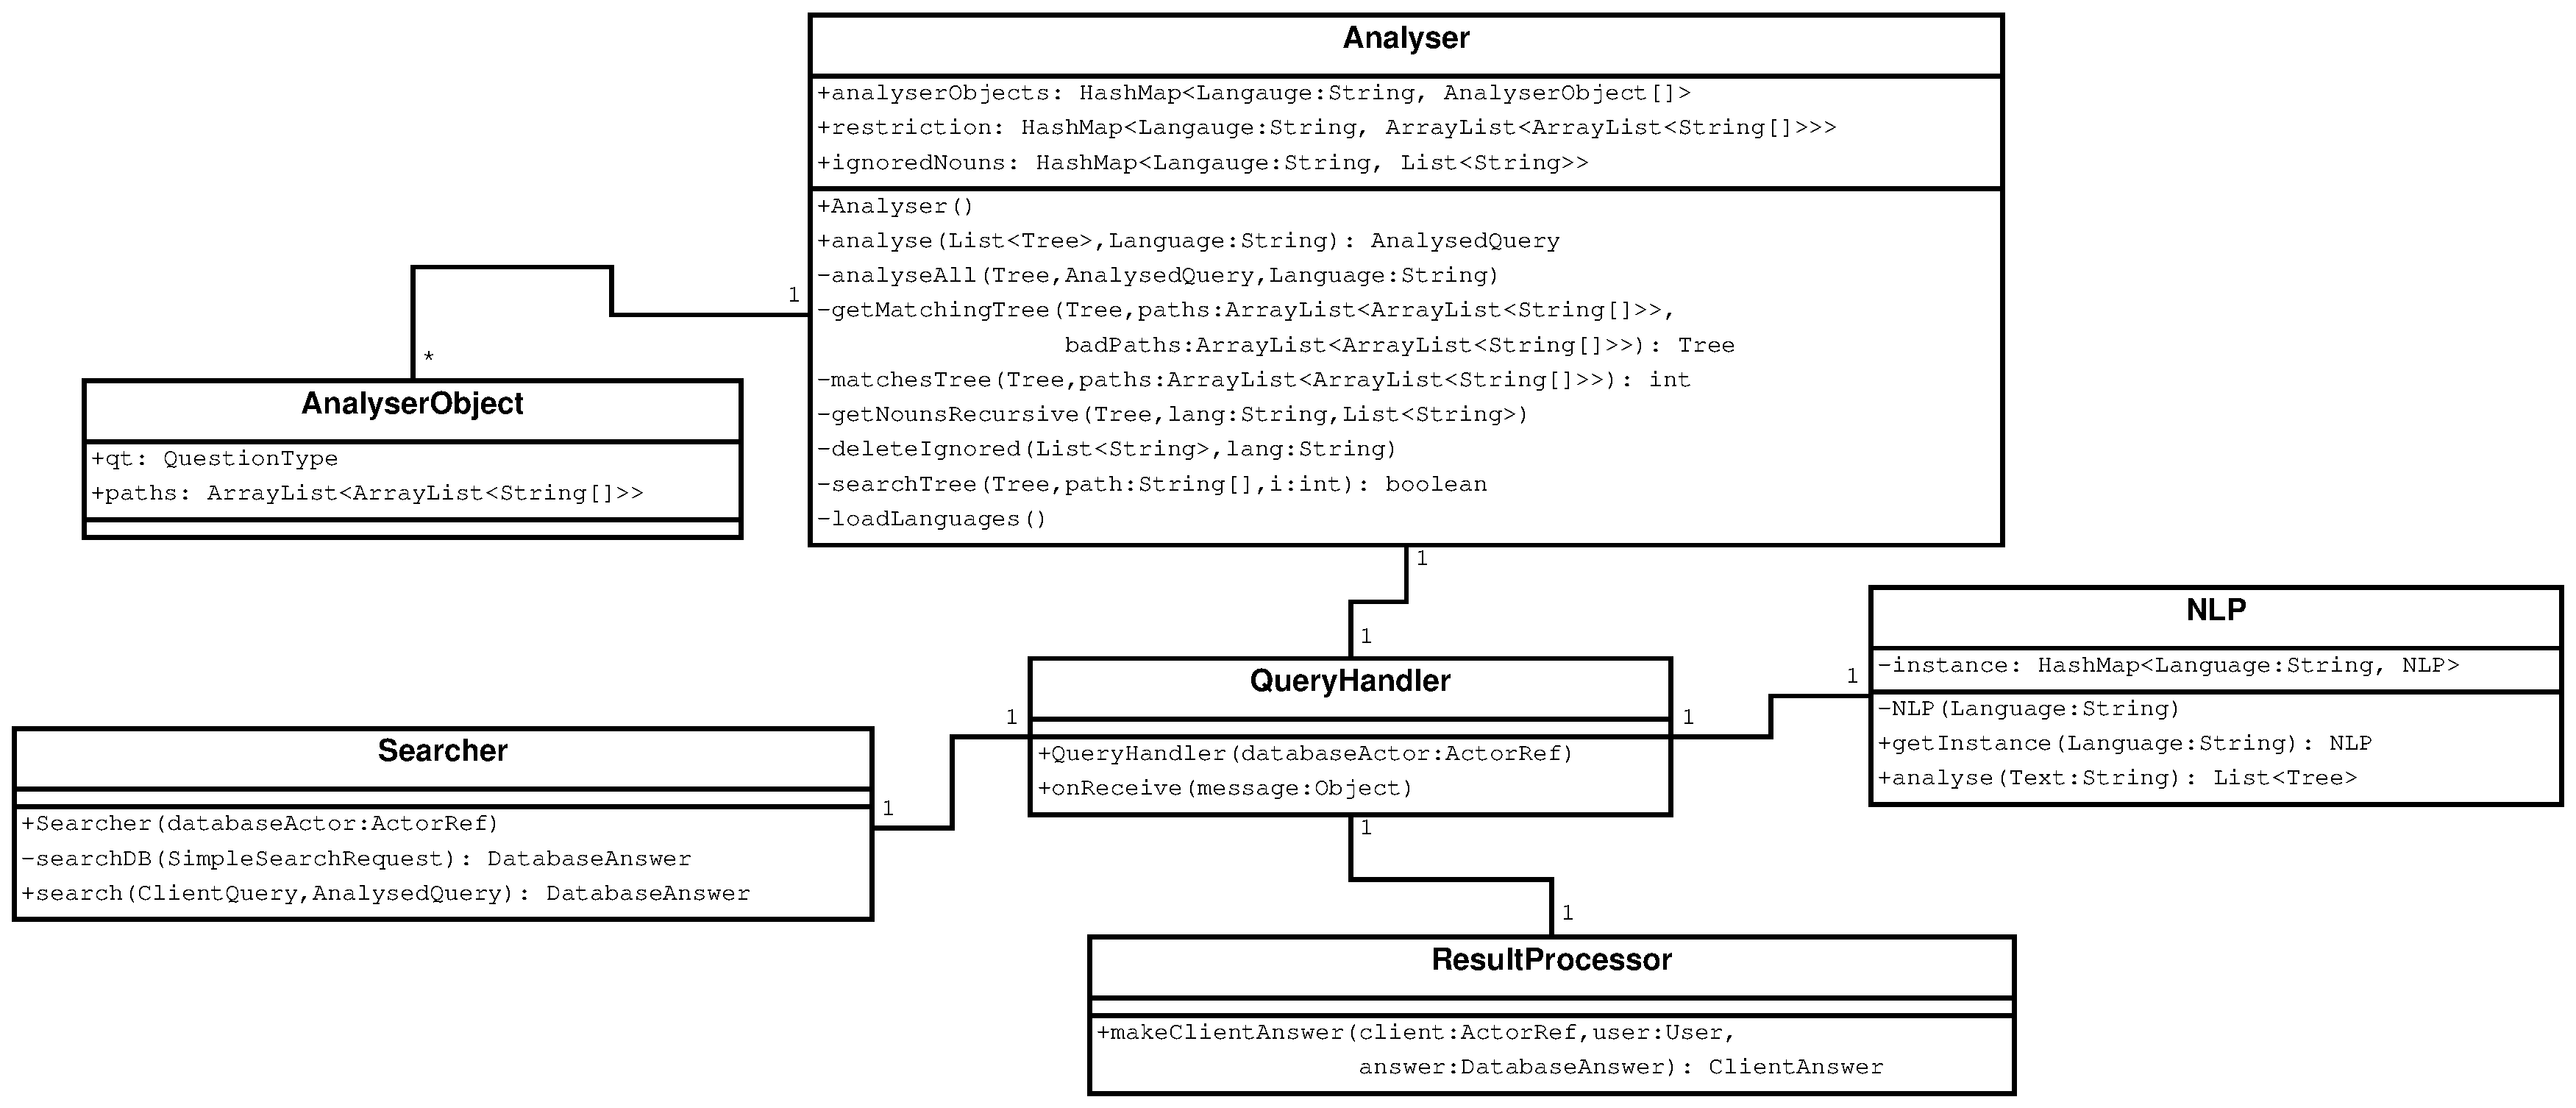
\includegraphics[width=1\textheight, angle=90]{Systementwurf/05_implementierungsentwurf/Diagramm1}
\caption{Klassendiagramm für Komponente \ref{C50}}
\end{figure}
 
\FloatBarrier

\subsection{Erläuterung}

Im Folgenden werden Attribute, Aufgaben und Kommunikationspartner für jede
Klasse der Serverkomponenten kurz erläutert. Triviale Methoden werden dabei
nicht berücksichtigt.

\begin{class}{50}{Analyser}
\item[Aufgabe]~\
Analysiert Wortbäume mit Suchmustern, durch die die gestellte Frage erkannt
werden kann.
\item[Attribute]~\
\begin{itemize}
\item \texttt{analyserObjects}: \texttt{HashMap<String, AnalyserObject[]>}:
Enthält zu einer Sprache AnalyserObjects.
\item \texttt{restriction}: \texttt{HashMap<String,
ArrayList<ArrayList<String[]>>>}: Enthält für eine Sprache Suchmuster für Restriktionen.
\item \texttt{ignoredNouns}: \texttt{HashMap<String, List<String>>}: Enthält
für eine Sprache eine Liste mit Wörter die ignoriert werden sollen.
\end{itemize}
\item[Operationen]~\
\begin{itemize}
\item \texttt{Analyser()}: Erstellt eine Instanz des Analysers.
\item \texttt{analyse(List<Tree> treeList)}: Analysiert eine Wort-Baum-Liste.
\item \texttt{analyseAll(Tree tree, AnalysedQuery analysedQuery, String lang)}:
Findet für einen gegebenen Wort-Baum eines Satzes in einer Sprache den Fragetyp und Schlüsselwörter heraus.
\item \texttt{getMatchingTree(Tree tree, ArrayList<ArrayList<String[]>> paths,
ArrayList<ArrayList<String[]>> badPaths)}: Sucht mithilfe eines gegebenen
Musters nach einer Struktur im Baum und gibt diese aus.
\item \texttt{matchesTree(Tree tree, ArrayList<ArrayList<String[]>> paths)}:
Prüft, ob ein Baum mit einem gegeben Muster übereinstimmt.
\item \texttt{getNounsRecursive(Tree tree, String lang, List<String> list)}:
Suche alle Nomen aus einem Baum heraus und fügt diese in eine Liste ein.
\item \texttt{deleteIgnored(List<String> list, String lang)}: Entfernt alle zu
ignorierende Wörter aus einer Liste.
\item \texttt{searchTree(Tree tree, String[] path, int i)}: Prüft, ob ein
gegebener Such-Pfad im Baum existiert.
\item \texttt{loadLanguages()}: Ließt Suchmuster einer Sprache in
AnalyserObject ein.
\end{itemize}
\item[Kommunikationspartner]~\
\textit{QueryHandler}
\end{class}

\begin{class}{50}{AnalysedObject}
\item[Aufgabe]~\
Enthält einen Fragetyp und ein Suchmuster, mit dem man den Fragetyp
identifizieren kann.
\item[Attribute]~\
\begin{itemize}
\item \texttt{qt}: \texttt{QuestionType} Der Fragetyp.
\item \texttt{paths}: \texttt{ArrayList<ArrayList<String[]>>} Das Suchmuster.
\end{itemize}
\item[Operationen]~\
keine
\item[Kommunikationspartner]~\
\textit{Analyser}
\end{class}

\begin{class}{50}{Searcher}
\item[Aufgabe]~\
Kommuniziert mit der Datenbank.
\item[Attribute]~\
keine
\item[Operationen]~\
\begin{itemize}
\item \texttt{Searcher(ActorRef databaseActor)}: Instanziert den Searcher
\item \texttt{search(Messages.ClientQuery originalQuery, AnalysedQuery aq)}:Sucht entsprechend der Fragestellung nach Ergebnissen.
\item \texttt{searchDB(SimpleSearchRequest simpleSearchRequest)}: Stellt anfragen an die Datenbank.
\end{itemize}
\item[Kommunikationspartner]~\
\textit{DatabaseHandler}, \textit{QueryHandler}
\end{class}

\begin{class}{50}{QueryHandler}
\item[Aufgabe]~\
Der QueryHandler organisiert die Analyse der Querries.
\item[Attribute]~\
keine
\item[Operationen]~\
\begin{itemize}
	\item \texttt{QueryHandler(ActorRef databaseActor)}: Instanziiert den QueryHandler.
	\item \texttt{onReceive(Object message)}: Nimmt ClientQuery-Nachrichten entgegen, und lässt diese analysieren.
\end{itemize}
\item[Kommunikationspartner]~\
\textit{NLP}, \textit{ManagementHandler}, \textit{Searcher}, \textit{ResultProcessor}, \textit{Analyser}
\end{class}

\begin{class}{50}{NLP}
\item[Aufgabe]~\
Zerlegt Texte in Wort-Bäume, die der Analyser verarbeiten kann.
\item[Attribute]~\
\begin{itemize}
\item \texttt{instance}: \texttt{HashMap<String, NLP>} Enthält die NLP Instanz einer Sprache.
\end{itemize}
\item[Operationen]~\
\begin{itemize}
\item \texttt{NLP(String lang)}: Instanziiert NLP für eine gegebene Sprache.
\item \texttt{getInstance(String lang)}: Gibt die NLP-Instanz der jeweiligen
Sprache aus.
\item \texttt{analyse(String text)}: Analysiert einen Text bezüglich seiner
Sprache und erstellt daraus eine Wort-Baumstruktur, in der die Bedeutung der
einzelner Wörter steht.
\end{itemize}
\item[Kommunikationspartner]~\
\textit{QueryHandler}
\end{class}

\begin{class}{50}{ResultProcessor}
\item[Aufgabe]~\
Generiert aus vorgefertigten Textbausteinen und
Ergebnissen eine Antwort.
\item[Attribute]~\ keine
\item[Operationen]~\
\begin{itemize}
\item \texttt{makeClientAnswer(ActorRef client, User user, DatabaseAnswer
answer)}: Produziert aus einer SearchAnswer eine ClientAnswer.
\end{itemize}
\item[Kommunikationspartner]~\
\textit{QueryHandler}
\end{class}
